% !TEX root = ../../thesis.tex
%______________________________________________________________________________
%
% SECTION
\section{The Spectral Element Method}
\label{section:sem}
%
%______________________________________________________________________________

As pointed out in section \ref{section:wave_equation}, a diagonal mass matrix $\mathbf M$ is essential to fully exploit the efficiency of explicit time integration schemes. A well-established approach that yields an inherently diagonal consistent mass matrix, is the Spectral Element Method (SEM) \cite{Maggio1994}. Based on the p-version of the FEM, the SEM relies on a specific choice of ansatz space and quadrature rule for its appealing properties.

Using the same line of thought as for the simplification of the moment fitting equations described in section \ref{section:fcm}, Lagrange polynomials defined on a set of Gauss-Lobatto points are used as basis functions. Accordingly, the quadrature rule for integrating the mass matrix is the Gauss-Lobatto scheme of matching order, which means that the integration points coincide with those used for the definition of the basis functions. As a result, the product of mixed ansatz functions vanish at all integration points, leading to a diagonal mass matrix.

\begin{equation}
	N_i(\boldsymbol{\xi}_k)N_j(\boldsymbol{\xi}_k) = 0 \ \ \forall i \neq j \ \ \forall k \in \{1..m\}
\end{equation}

\begin{equation}
	M_{ij} = \int_{\Omega} N_i \rho N_j d\mathbf x
	\approx
	det(\mathbf J) \sum_{k=1}^m N_i(\boldsymbol{\xi}_k) \rho N_j(\boldsymbol{\xi}_k) w_k
	=
	\begin{bmatrix}
		M_{11} & & 0 \\
		& \ddots & \\
		0 & & M_{nn} \\
	\end{bmatrix}
\end{equation}

where $\mathbf J$ is the Jacobian facilitating the change of variables from $\mathbf x$ to $\boldsymbol{\xi}$.

Gauss-Lobatto points are chosen in particular because they always include the limits of the integration domain $-1$ and $1$, ensuring that all except one ansatz functions vanish on each border, as shown in figure \ref{fig:lagrange_basis}. This property is essential for FE-based methods to ensure the continuity between elements, allow the blending of specific ansatz functions to exactly capture boundaries, and strongly enforce boundary conditions.

\begin{figure}[h]
	\centering
	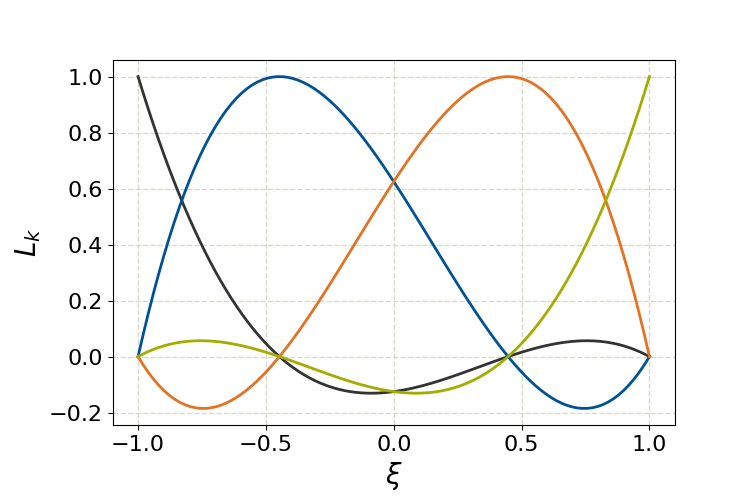
\includegraphics[height=6cm]{pictures/figures/lagrange_basis.png}
	\caption{Lagrange basis functions on a set of fourth order Gauss-Lobatto points.}
	\label{fig:lagrange_basis}
\end{figure}

Using a Lagrange basis instead of integrated Legendre polynomials has numerous additional consequences, most of them undesirable. Firstly, the hierarchic nature of the ansatz space is lost, requiring the re-evaluation of the entire stiffness matrix as well when performing p-refinement. Moreover, the conditioning of the stiffness matrix is worse \cite{Zumbusch1996}, and degrades more rapidly with increasing $p$. Lastly, no complete trunk space of Lagrange polynomials exist, which means that the ansatz space must be constructed from the tensor product of the basis functions, leading to an increased number of degrees of freedom and requiring more computational resources. Lastly, constructing ansatz spaces with inhomogeneous polynomial orders is more complicated than it is for hierarchic basis functions.
On the other hand, Lagrange basis functions are nodal and have a partition of unity $\sum_{k=1}^m L_k(\xi) = 1$.

To ensure the diagonality of the mass matrix, the basis functions' polynomial order $p$ enforces the quadrature scheme to be the tensor product of the $m=p+1$ order Gauss-Lobatto rule, leading to further undesirable effects. The most obvious one of course is the lack of choice when it comes to the selection of integration schemes. This ties the integration order to the order of the basis functions regardless of the order of the integrands in equation \ref{eq:structural_components}, meaning that integration errors increase with the order of material parameters. The highest polynomial order a tensor product quadrature scheme is able to exactly integrate is identical to that of the underlying 1D rule for each variable \cite{Keister1996}. In the case of SEM, this translates to $2m-3=2p-1$. Considering \ref{eq:structural_components}, the highest order of the mass matrix's integrand is $2p$ per direction, while the stiffness matrix's is $2p-1$ in 1D and $2p$ in higher dimensions. Consequently, neither the mass nor the stiffness matrix can be integrated exactly (apart from 1D models), even for constant material parameters.

Since no benefit is gained by using the Gauss-Lobatto rule for the stiffness matrix and load vector, a different integration scheme can be applied. Unfortunately, no solution exists to this problem in the mass matrix's case, meaning that it is always underintegrated in the SEM. It is important to note that under certain circumstances, especially in wave propagation problems, this drawback partly balances other errors originating from the discretization \cite{Ainsworth2010}, leading to more accurate results when compared to the classical FEM. In general however, it is an additional source of errors that increase with the order of the density function.